\documentclass{article}

\usepackage{listings}
\usepackage{xcolor}
\usepackage{graphicx}
\usepackage{subcaption}

\newcommand{\BeginThingTaxonomy}{4}
\newcommand{\EndThingTaxonomy}{49}
\newcommand{\BeginAbstractIndividualTaxonomy}{51}
\newcommand{\EndAbstractIndividualTaxonomy}{86}
\newcommand{\BeginEndurantTaxonomy}{88}
\newcommand{\EndEndurantTaxonomy}{145}
\newcommand{\BeginEndurantTaxonomyOfNaturesBegin}{147}
\newcommand{\EndEndurantTaxonomyOfNaturesEnd}{192}
\newcommand{\BeginEndurantTaxonomyOfPropertiesBegin}{194}
\newcommand{\EndEndurantTaxonomyOfPropertiesEnd}{271}
\newcommand{\BeginInstantationAndSpecialzation}{273}
\newcommand{\EndInstantationAndSpecialzation}{356}
\newcommand{\BeginRigidityAndSortality}{360}
\newcommand{\EndRigidityAndSortality}{626}
\newcommand{\BeginEndurantsTypesDefinition}{628}
\newcommand{\EndEndurantsTypesDefinition}{835}
\newcommand{\BeginMereology}{837}
\newcommand{\EndMereology}{888}
\newcommand{\BeginComposition}{886}
\newcommand{\EndComposition}{914}
\newcommand{\BeginConstitution}{916}
\newcommand{\EndConstitution}{959}
\newcommand{\BeginExistentialDependence}{961}
\newcommand{\EndExistentialDependence}{983}
\newcommand{\BeginMomentsAndInherence}{985}
\newcommand{\EndMomentsAndInherence}{1055}
\newcommand{\BeginRelators}{1057}
\newcommand{\EndRelators}{1137}
\newcommand{\BeginCharacterization}{1139}
\newcommand{\EndCharacterization}{1156}
\newcommand{\BeginQualitiesAndQualityStructures}{1162}
\newcommand{\EndQualitiesAndQualityStructures}{1180}
\newcommand{\BeginEndurantsAndPerdurants}{1182}
\newcommand{\EndEndurantsAndPerdurants}{1201}

% newcommand for labels of axioms, theorems and definitions
\newcommand{\AxLabel}{a}
\newcommand{\ThLabel}{t}

% counter and newcommand for numbering formulas
\newcounter{cntax}
\newcommand{\myax}[1]{\refstepcounter{cntax}{\bf \small \AxLabel\thecntax}\label{#1}$\,\,\,\,$}
\newcounter{cntth}
\newcommand{\myth}[1]{\refstepcounter{cntth}{\bf \small \ThLabel\thecntth}\label{#1}$\,\,\,\,$}

% newcommands to refer to formulas with labels
\newcommand{\refax}[1]{(\AxLabel\ref{#1})}
\newcommand{\refth}[1]{(\ThLabel\ref{#1})}

\definecolor{codegreen}{rgb}{0,0.6,0}
\definecolor{codegray}{rgb}{0.5,0.5,0.5}
\definecolor{codepurple}{rgb}{0.58,0,0.82}
\definecolor{backcolour}{rgb}{0.95,0.95,0.92}

\lstdefinestyle{mystyle}{
    backgroundcolor=\color{backcolour},
    commentstyle=\color{codegreen},
    keywordstyle=\color{magenta},
    numberstyle=\tiny\color{codegray},
    stringstyle=\color{codepurple},
    basicstyle=\ttfamily\footnotesize,
    breaklines=true,
    keepspaces=true,
    numbers=left,
    numbersep=5pt,
    showspaces=false,
    showstringspaces=false,
    showtabs=false,
    tabsize=2
}

\lstset{style=mystyle}

\title{A First-Order Logic Formalization of the Unified Foundational Ontology}
\author{
    Daniele Porelo,
    Claudenir M. Fonseca,
    Jo\~ao Paulo A. Almeida,\\
    Giancarlo Guizzardi,
    Tiago Prince Sales
}
\date{\today}

\begin{document}
\maketitle

\begin{abstract}
This document presents a formalization of the Unified Foundational Ontology (UFO) in first-order logic. This formalization is documented by means of three complementary representations: (i) a representation in standard Common Logic using the CLIF syntax; (ii) a representation in natural language; and, when applicable, a (iii) UML-based diagrammatic representation. The presented formalization is supported by consistency and satisfiability checks performed through automated proofing tools.
\end{abstract}

\section{Introduction}

This document presents a formalization of the Unified Foundational Ontology (UFO) in first-order logic. This formalization is documented by means of three complementary representations: (i) a representation in standard Common Logic using the CLIF syntax; (ii) a representation in natural language; and, when applicable, a (iii) UML-based diagrammatic representation. The presented formalization is supported by consistency and satisfiability checks performed through automated proofing tools.

The remainder of this document is organized as a single formalization section (Section~\ref{sec:formalization}), which contains subsections for each submodule of the ontology.

\section{Formalization}
\label{sec:formalization}

This section contains the formalization of the Unified Foundational Ontology (UFO) in first-order logics. This formalization is organized in several subsections where each presents the formalization of a portion of the whole ontology. The formalization is presented through different equivalent representations, designed to support the understanding of its contents: (i) a representation in standard Common Logic using the CLIF syntax; (ii) a representation in natural language; and, when applicable, a (iii) UML-based diagrammatic representation.

The UML-based diagrammatic representation serves as a visual representation certain predicates and axioms, being each element in Figure~\ref{fig:diagram_conventions} being translated as follows:

\begin{figure}
    \centering
    \begin{subfigure}[b]{0.3\textwidth}
        \centering
        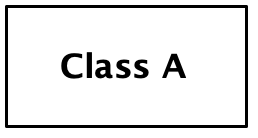
\includegraphics[width=0.5\textwidth]{diagrams/Conventions_Class.png}
        \caption{Rectangle shape.}
        \label{fig:diagram_conventions_rectangle}
    \end{subfigure}
    \qquad
    \centering
    \begin{subfigure}[b]{0.45\textwidth}
        \centering
        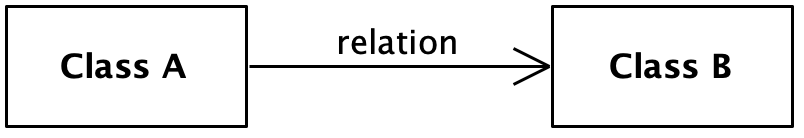
\includegraphics[width=\textwidth]{diagrams/Conventions_Relation.png}
        \caption{Labeled open arrow.}
        \label{fig:diagram_conventions_open_arrow}
    \end{subfigure}
    
    \centering
    \begin{subfigure}[b]{0.3\textwidth}
        \centering
        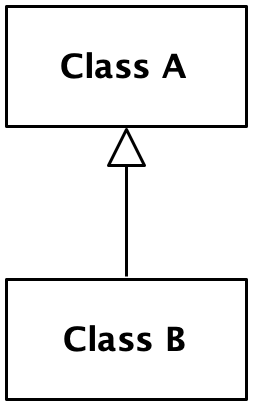
\includegraphics[width=0.5\textwidth]{diagrams/Conventions_Specialization.png}
        \caption{Closed arrow.}
        \label{fig:diagram_conventions_closed_arrow}
    \end{subfigure}
    \qquad
    \centering
    \begin{subfigure}[b]{0.35\textwidth}
        \centering
        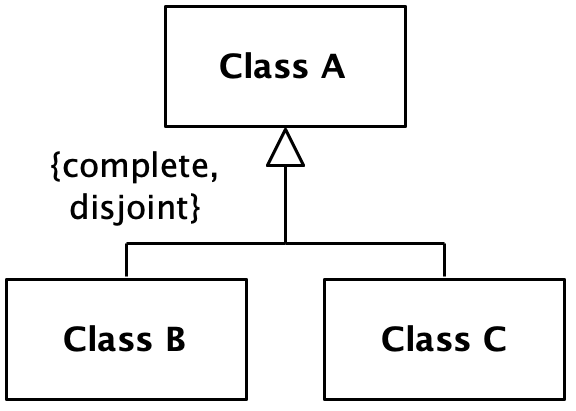
\includegraphics[width=\textwidth]{diagrams/Conventions_Generalization_Set.png}
        \caption{Labeled closed arrows.}
        \label{fig:diagram_conventions_labeled_arrow}
    \end{subfigure}
    \caption{UML-based representation of first-order logic axioms.}\label{fig:diagram_conventions}
\end{figure}

\begin{itemize}
    \item Rectangle shape (Figure~\ref{fig:diagram_conventions_rectangle}): visual representation of unary predicates associated to types in the ontology; the associated predicate is shown in lower camel case with no spaces.
    
    $classA(x)$

    \item Open arrow (Figure~\ref{fig:diagram_conventions_open_arrow}): visual representation of binary predicates; the predicate associated to the arrows' label is shown in lower camel case with no spaces; the predicate can only be true for any $x$ and $y$ if it is also true predicates associated to the types of each end (keeping the order of the arrow in the binary predicate's positions); this representation may also be associated to ternary predicates ifif its third position represents a time-index.
    
    $\forall x,y (relation(x,y) \rightarrow (classA(x) \wedge classB(y)))$
    
    $\forall x,y,w (relation(x,y,w) \rightarrow (classA(x) \wedge classB(y) \wedge world(w)))$

    \item Closed arrow (Figure~\ref{fig:diagram_conventions_closed_arrow}): visual representation of specializations between ontology's types, where the type in the tail of the arrow is a subtype of the type in the head of the arrow.
    
    $\forall x (classB(x) \rightarrow classA(x))$

    \item Labeled closed arrow (Figure~\ref{fig:diagram_conventions_labeled_arrow}): visual representation of disjoint and/or complete constraints over sets specializations between ontology's types.
    
    $\forall x (classB(x) \rightarrow classA(x))$\\
    $\forall x (classC(x) \rightarrow classA(x))$\\
    $\forall x (classA(x) \rightarrow (classB(x) \vee classC(x)))$  \hfill \{complete\}\\
    $\neg\exists x (classB(x) \wedge classC(x))$  \hfill \{disjoint\}
\end{itemize}

\subsection{UFO Taxonomy}

% Thing Taxonomy
\subsubsection{Partial Taxonomy of Thing}

\begin{figure}[ht]
    \centering
    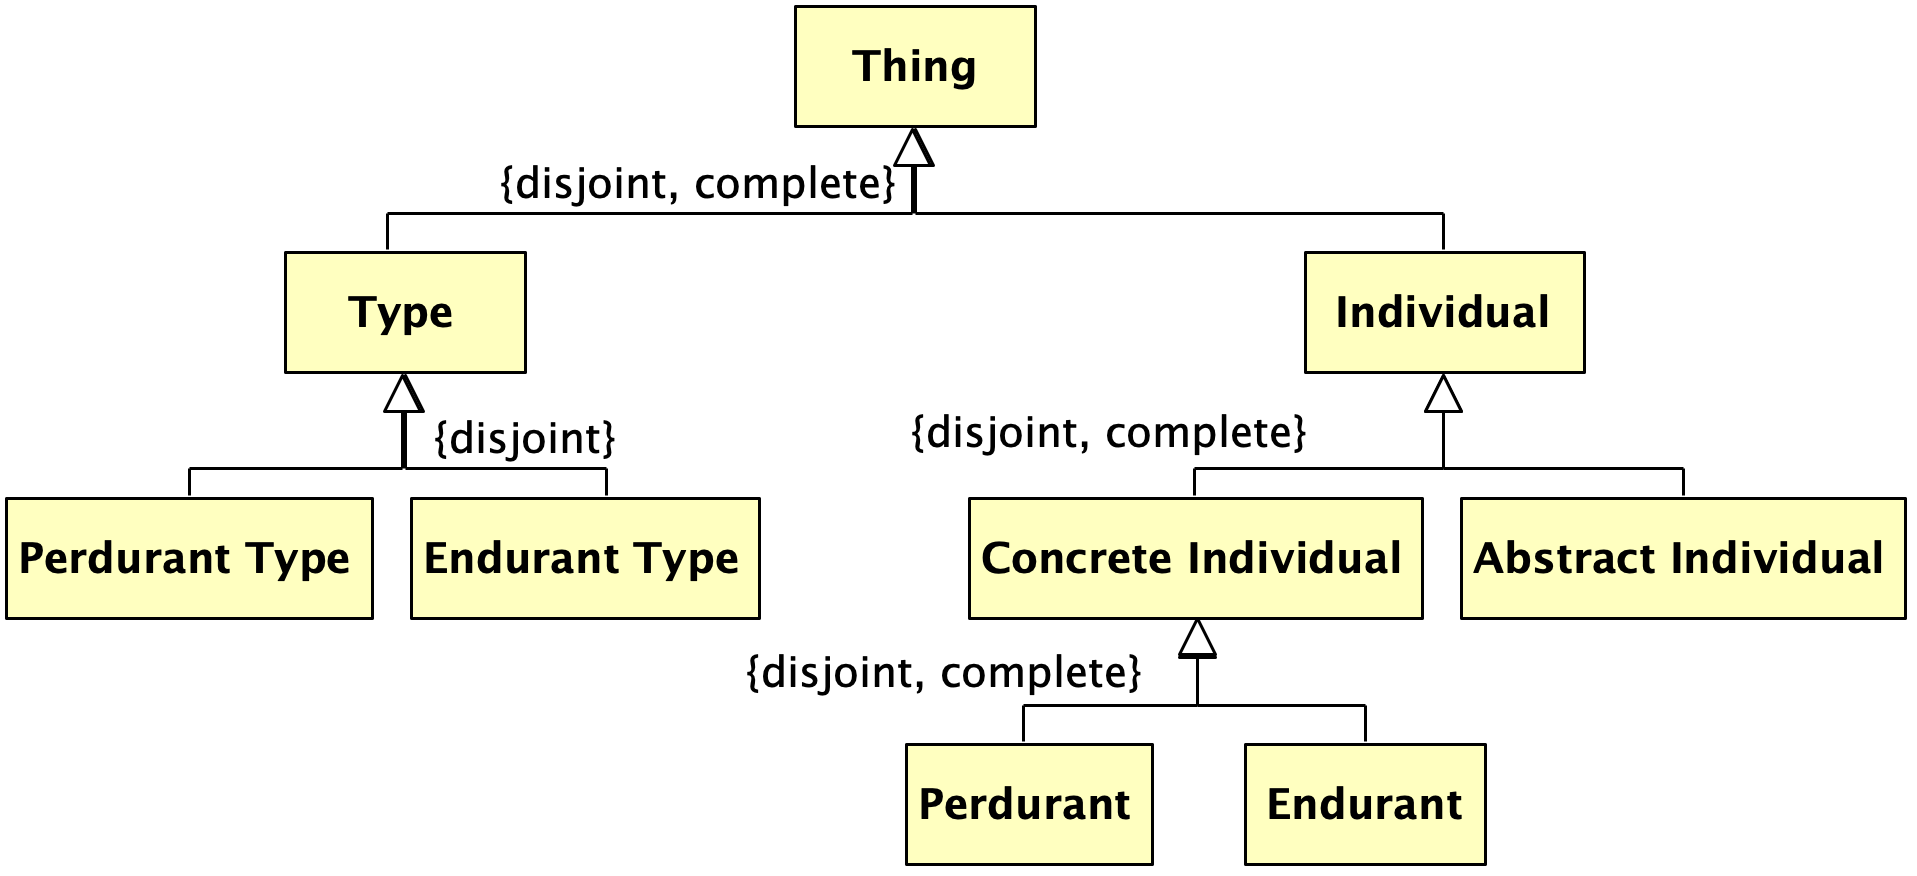
\includegraphics[width=0.8\textwidth]{diagrams/Thing_Diagram.png}
    \caption{Partial Taxonomy of UFO -- Thing.}
    \label{fig:ufo_taxonomy_thing}
\end{figure}

\lstinputlisting[
    firstline=\BeginThingTaxonomy,
    lastline=\EndThingTaxonomy,
    firstnumber=\BeginThingTaxonomy
]{ufo_2021.tex}

% Abstract Individual Taxonomy
\subsubsection{Partial Taxonomy of Abstract Individual}

% TODO: update taxonomy with a disjointness declaration between Quale, Set, and World
% Add World to the taxonomy

\begin{figure}[ht]
    \centering
    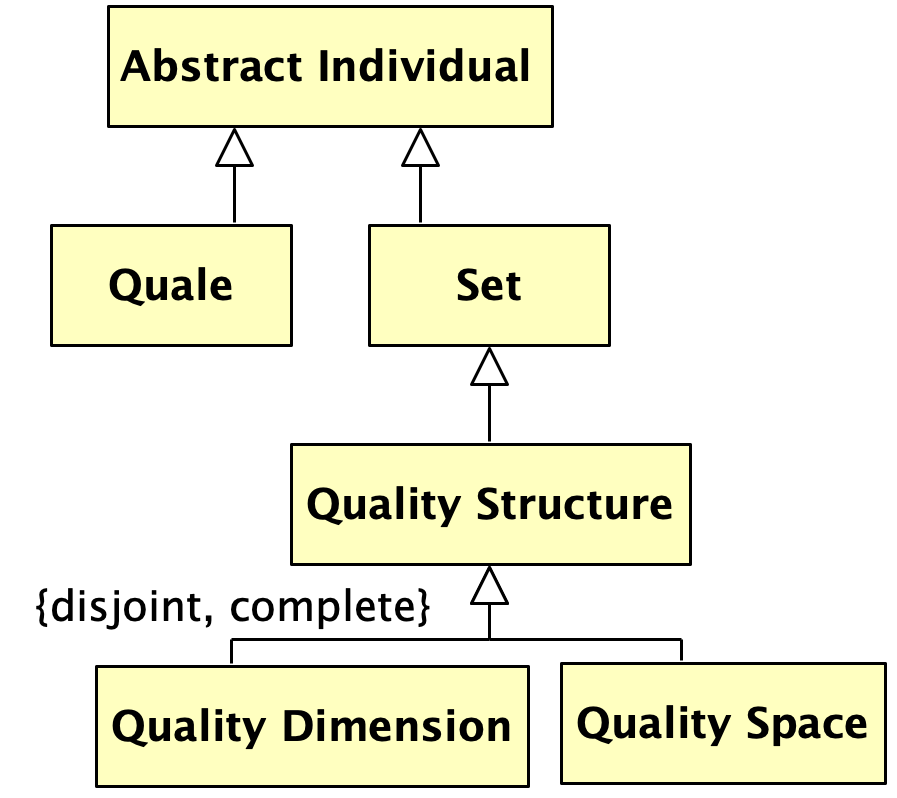
\includegraphics[width=0.4\textwidth]{diagrams/Abstract_Individual_Diagram.png}
    \caption{Partial Taxonomy of UFO -- Abstract Individual.}
    \label{fig:ufo_taxonomy_abstract_individual}
\end{figure}

\lstinputlisting[
    firstline=\BeginAbstractIndividualTaxonomy,
    lastline=\EndAbstractIndividualTaxonomy,
    firstnumber=\BeginAbstractIndividualTaxonomy 
]{ufo_2021.tex}

% Endurant Taxonomy
\subsubsection{Partial Taxonomy of Endurant}

\begin{figure}[ht]
    \centering
    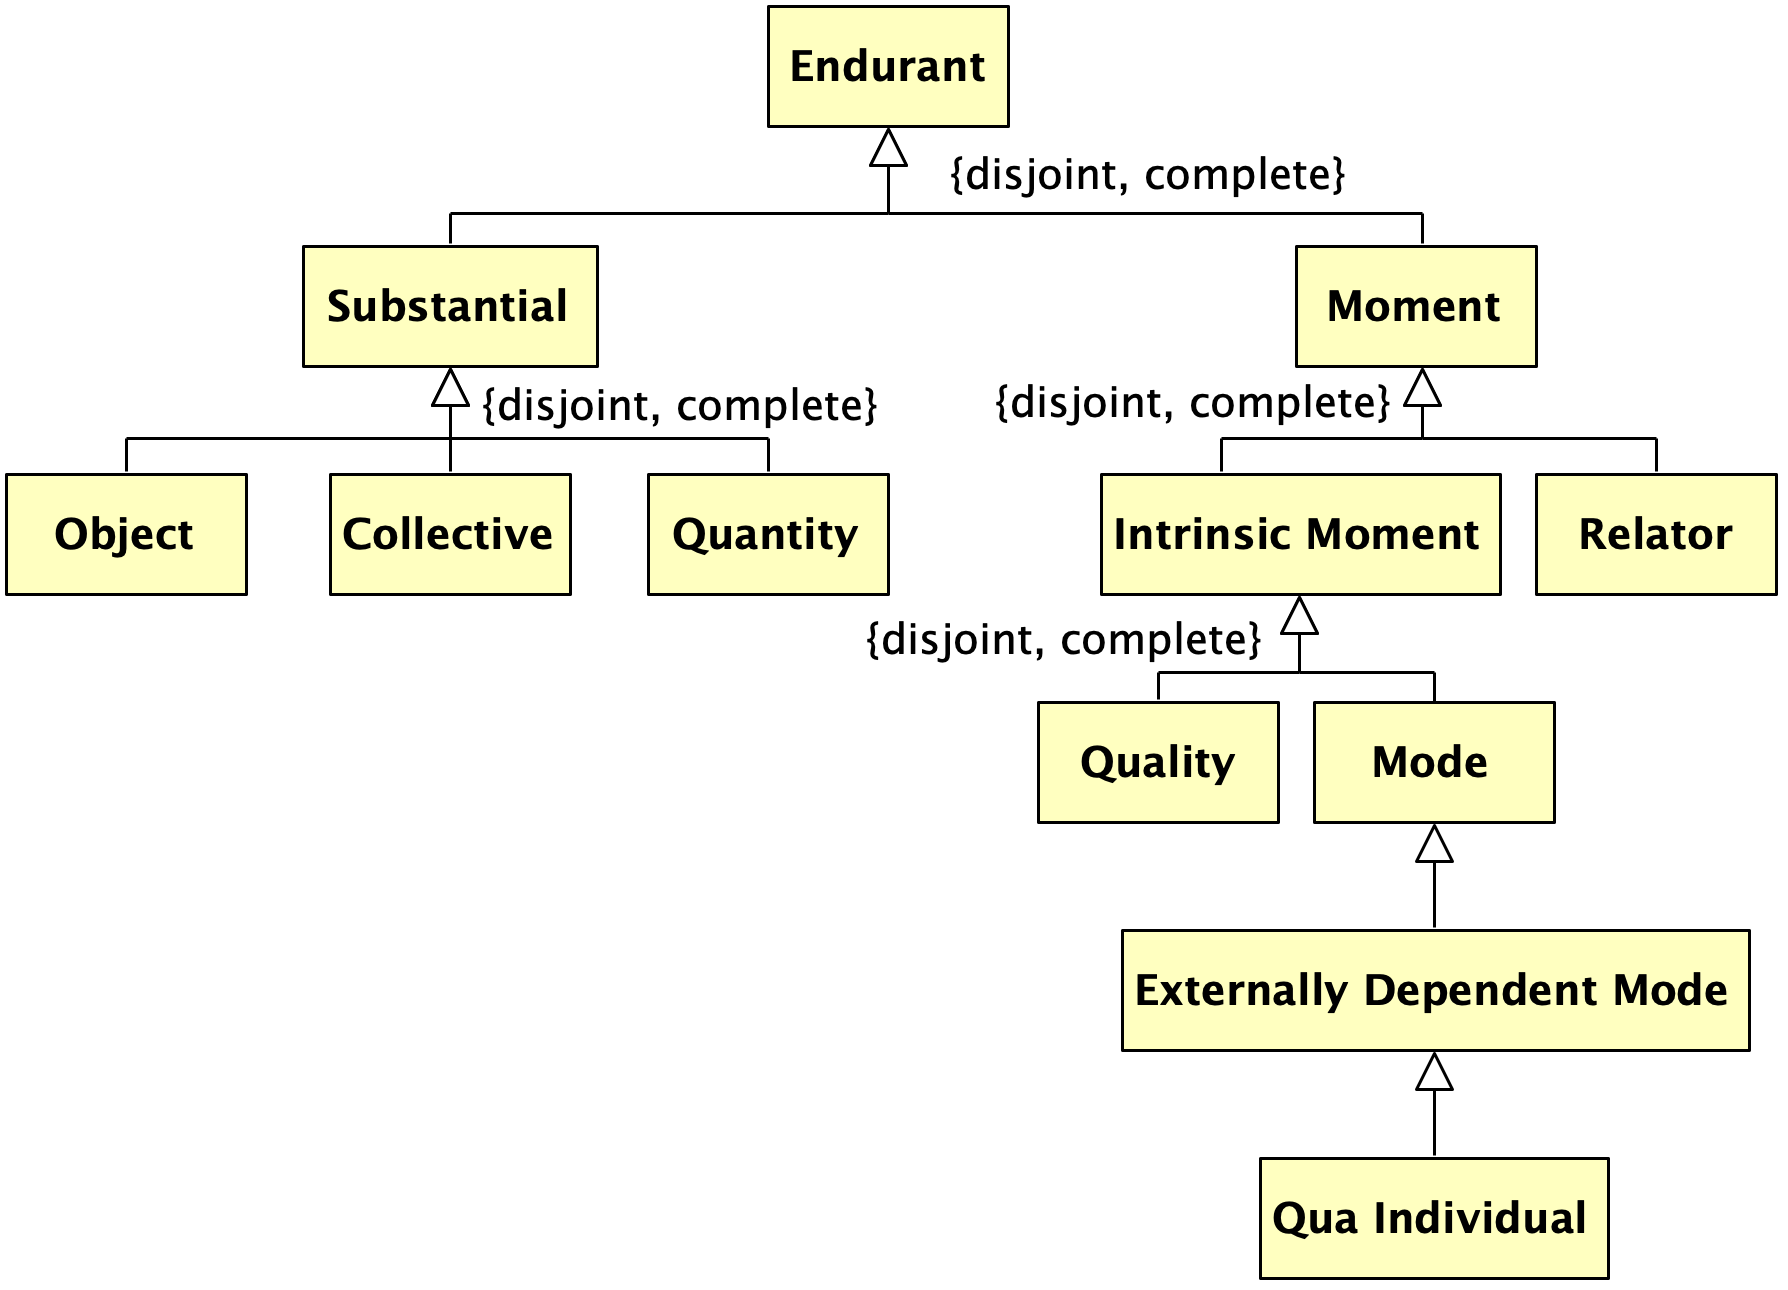
\includegraphics[width=0.8\textwidth]{diagrams/Endurant_Diagram.png}
    \caption{Partial Taxonomy of UFO -- Endurant.}
    \label{fig:ufo_taxonomy_endurant}
\end{figure}

\lstinputlisting[
    firstline=\BeginEndurantTaxonomy,
    lastline=\EndEndurantTaxonomy,
    firstnumber=\BeginEndurantTaxonomy,
]{ufo_2021.tex}

% Endurant Type Taxonomy of Ontological Natures
\subsubsection{Partial Taxonomy of Endurant Type (on ontological natures)}

\begin{figure}[ht]
    \centering
    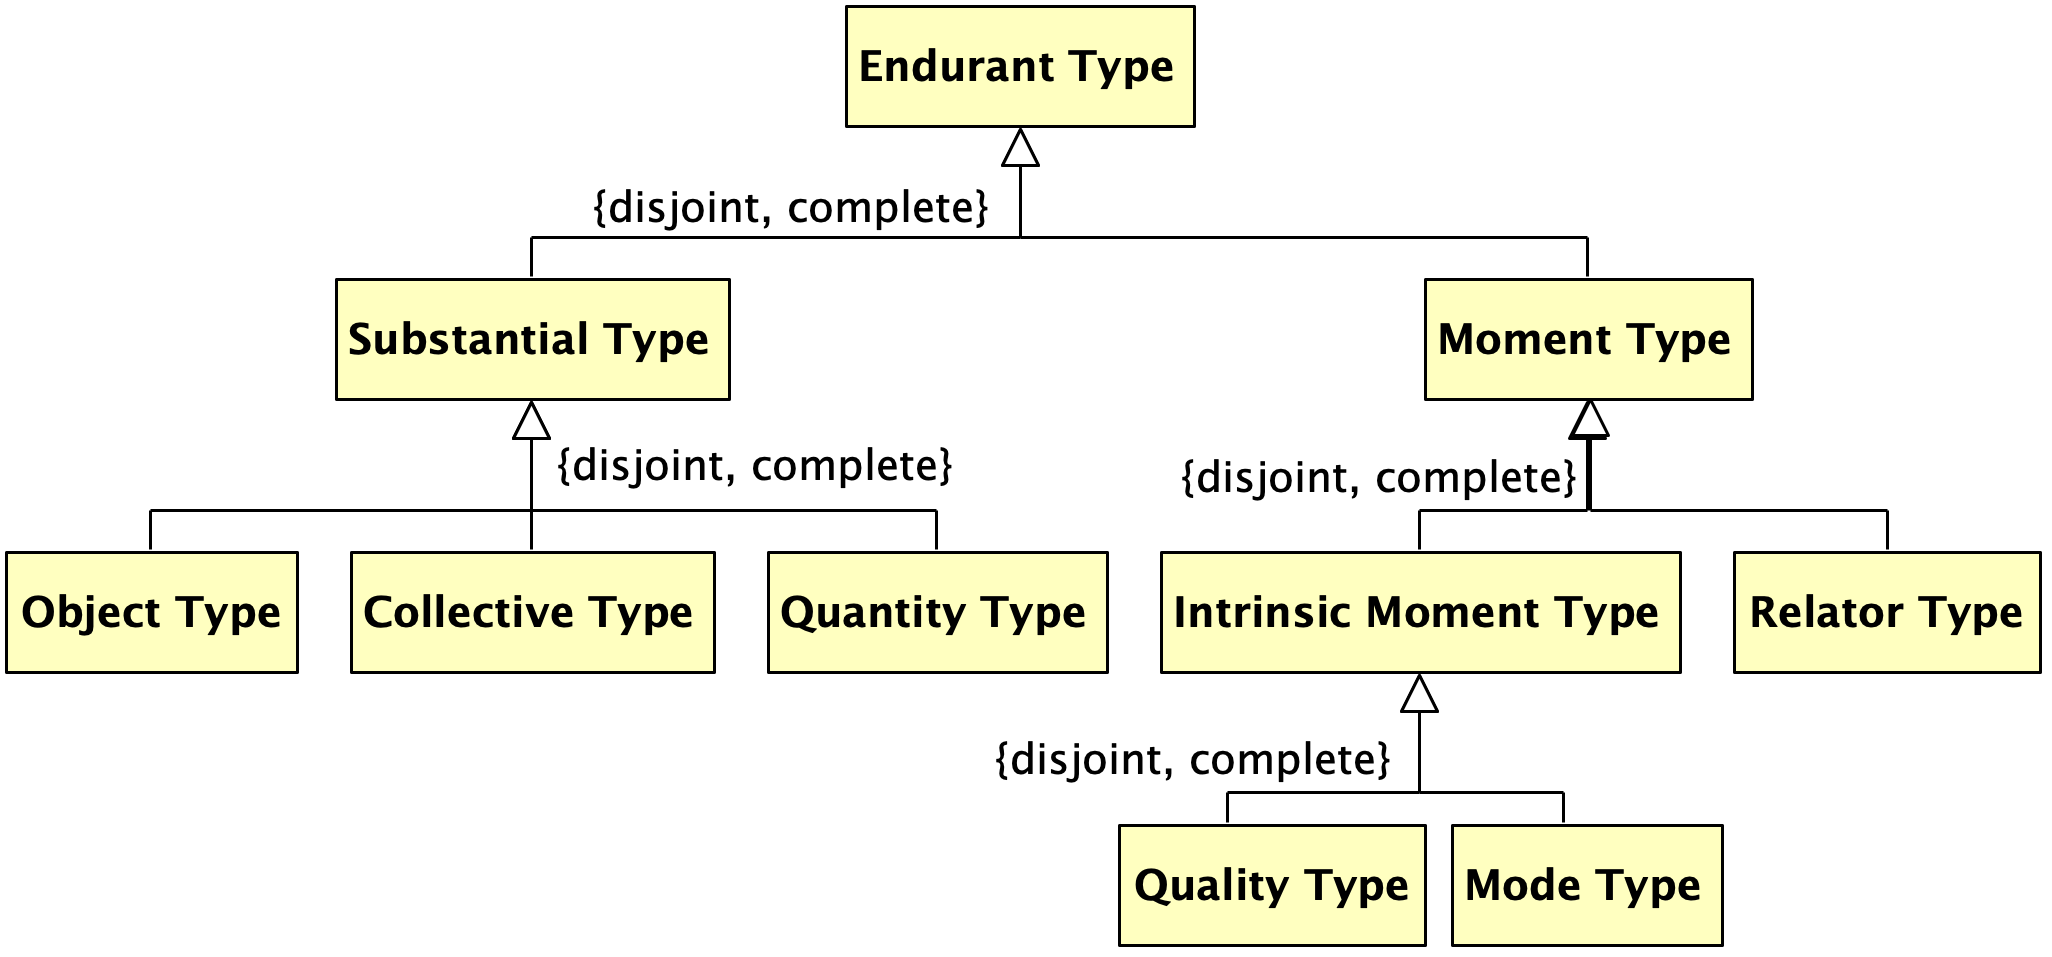
\includegraphics[width=0.9\textwidth]{diagrams/Endurant_Type_Natures_Diagram.png}
    \caption{Partial Taxonomy of UFO -- Endurant Types (by ontological nature).}
    \label{fig:ufo_taxonomy_endurant_types_natures}
\end{figure}

\lstinputlisting[
    firstline=\BeginEndurantTaxonomyOfNaturesBegin,
    lastline=\EndEndurantTaxonomyOfNaturesEnd,
    firstnumber=\BeginEndurantTaxonomyOfNaturesBegin
]{ufo_2021.tex}

% Endurant Type Taxonomy of Modal Properties of Types
\subsubsection{Partial Taxonomy of Endurant Type (on modal properties of types)}

\begin{figure}[ht]
    \centering
    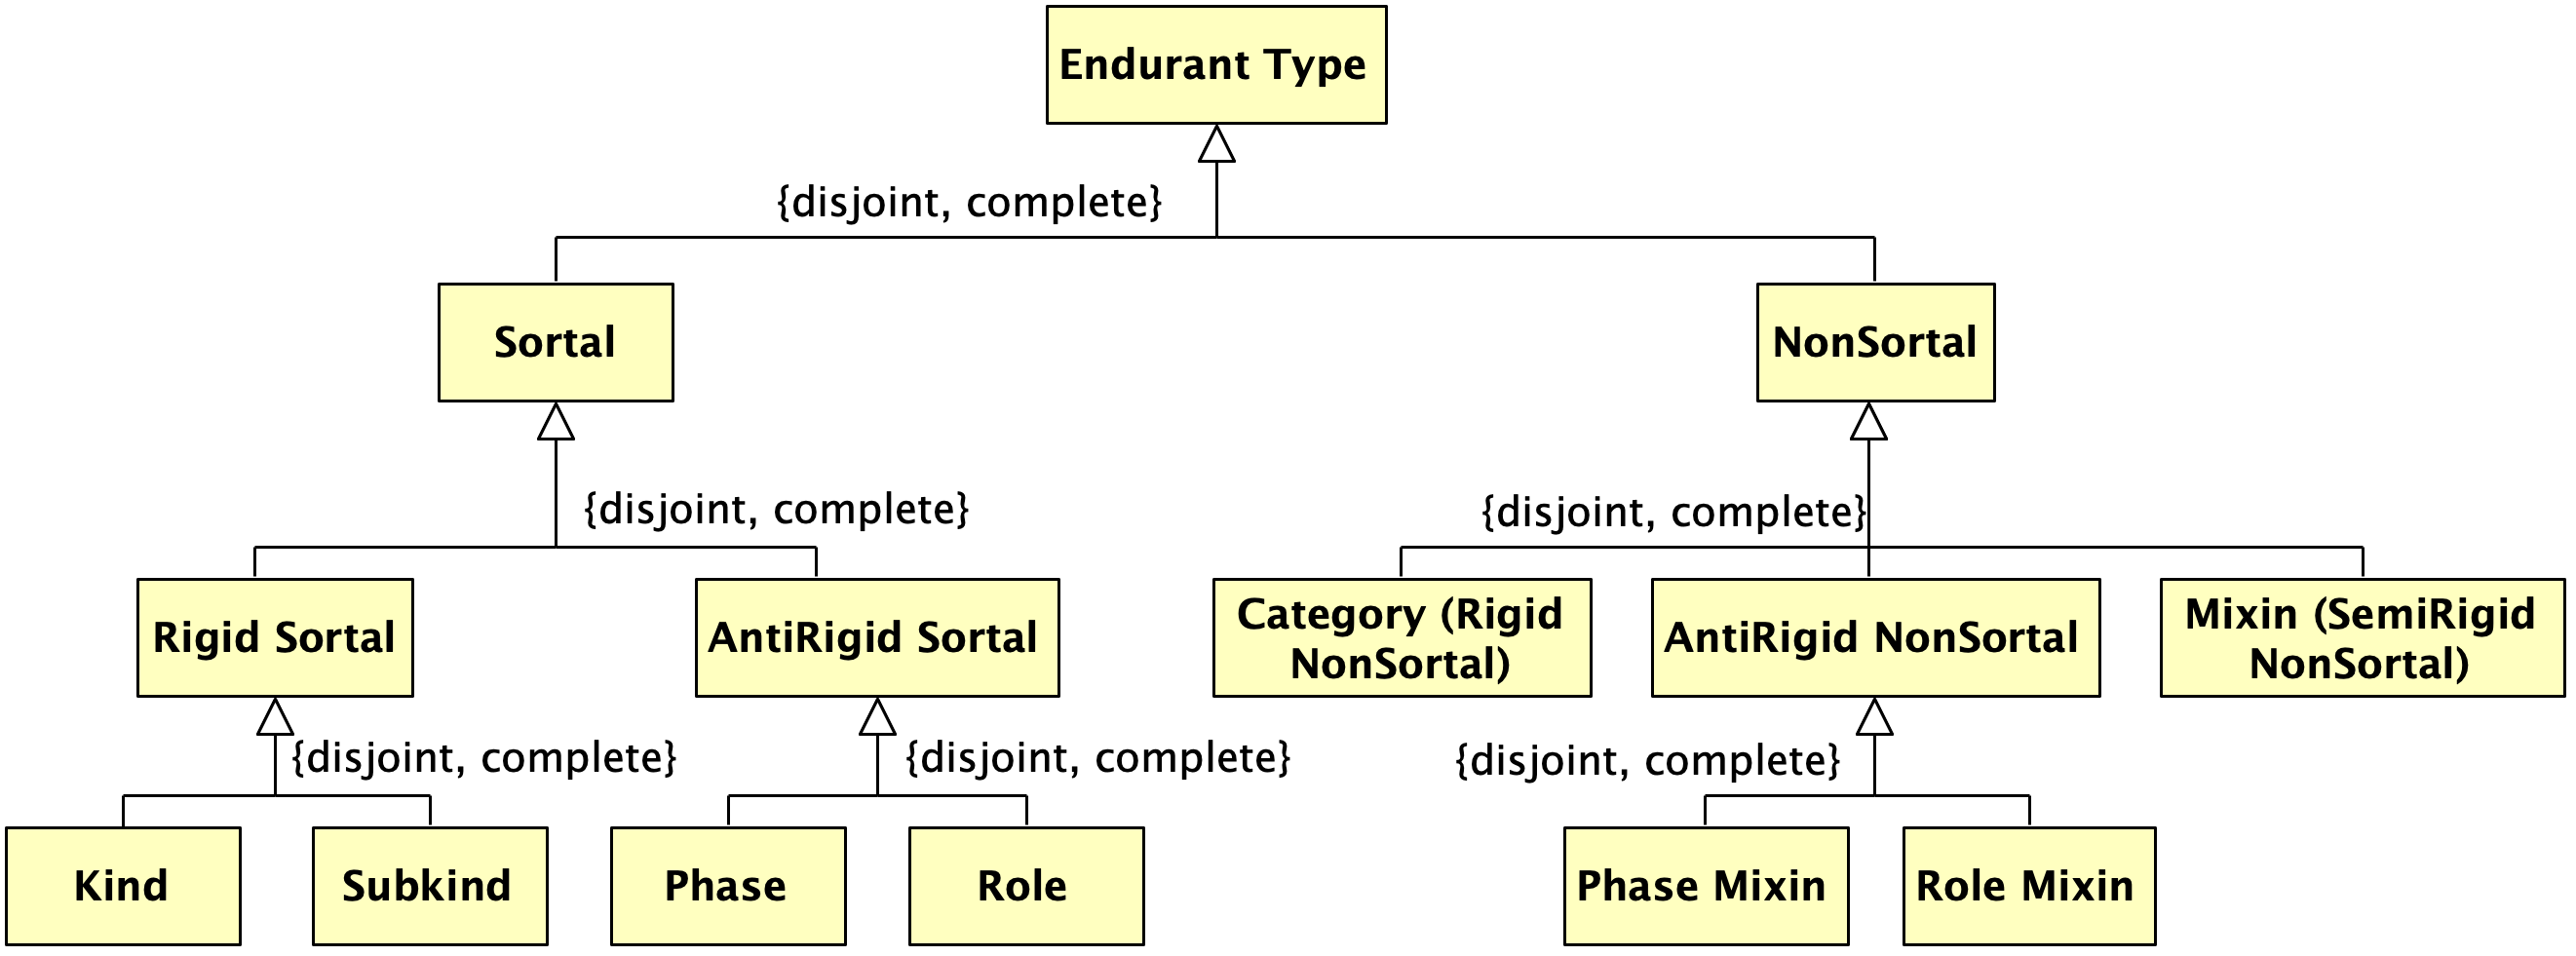
\includegraphics[width=\textwidth]{diagrams/Endurant_Type_Properties_Diagram.png}
    \caption{Partial Taxonomy of UFO -- Endurant Types (by modal properties of types).}
    \label{fig:ufo_taxonomy_endurant_types_properties}
\end{figure}

\lstinputlisting[
    firstline=\BeginEndurantTaxonomyOfPropertiesBegin, 
    lastline=\EndEndurantTaxonomyOfPropertiesEnd, 
    firstnumber=\BeginEndurantTaxonomyOfPropertiesBegin
]{ufo_2021.tex}

% Types, Individuals, Instantiation, and Specialization
\subsubsection{Defining Types, Individuals, and Specialization}

\begin{figure}[ht]
    \centering
    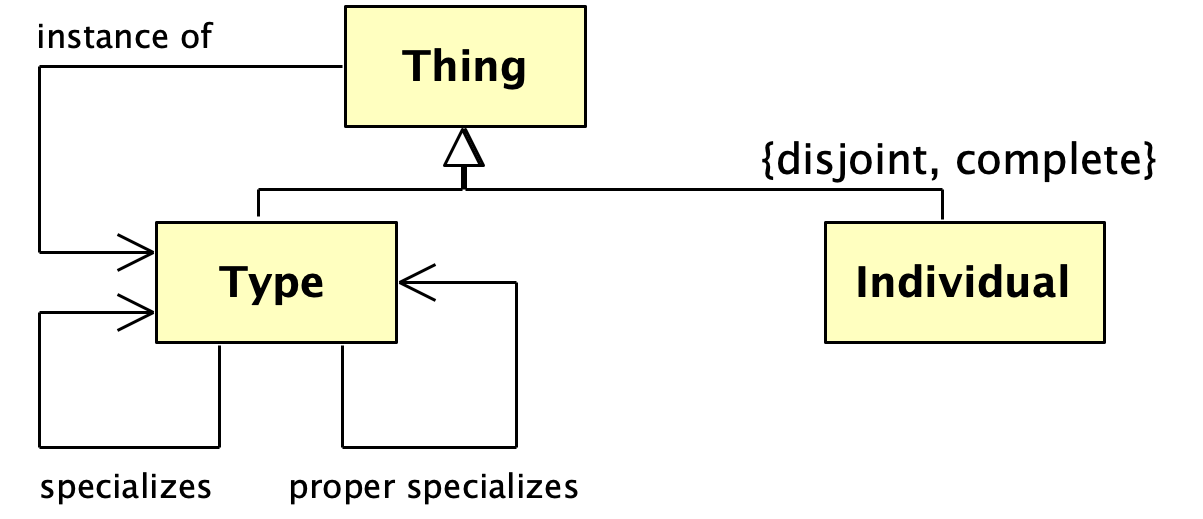
\includegraphics[width=0.6\textwidth]{diagrams/Instantiation_Diagram.png}
    \caption{Types, individuals, instantiation, and specialization.}
    \label{fig:instantiation_and_specialization}
\end{figure}

\lstinputlisting[
    firstline=\BeginInstantationAndSpecialzation, 
    lastline=\EndInstantationAndSpecialzation, 
    firstnumber=\BeginInstantationAndSpecialzation
]{ufo_2021.tex}

% Sortality and Rigidity
\subsubsection{Defining Rigidity and Sortality}

\lstinputlisting[
    firstline=\BeginRigidityAndSortality, 
    lastline=\EndRigidityAndSortality, 
    firstnumber=\BeginRigidityAndSortality
]{ufo_2021.tex}

% Endurant Types Definition
\subsubsection{Defining Endurant Types}

\lstinputlisting[
    firstline=\BeginEndurantsTypesDefinition, 
    lastline=\EndEndurantsTypesDefinition, 
    firstnumber=\BeginEndurantsTypesDefinition
]{ufo_2021.tex}

% Mereology
\subsubsection{Mereology}

\lstinputlisting[
    firstline=\BeginMereology, 
    lastline=\EndMereology, 
    firstnumber=\BeginMereology
]{ufo_2021.tex}

% Composition
\subsubsection{Composition}

\lstinputlisting[
    firstline=\BeginComposition, 
    lastline=\EndComposition, 
    firstnumber=\BeginComposition
]{ufo_2021.tex}

% Constitution
\subsubsection{Constitution}

\lstinputlisting[
    firstline=\BeginConstitution, 
    lastline=\EndConstitution, 
    firstnumber=\BeginConstitution
]{ufo_2021.tex}

% Existential Dependence
\subsubsection{Existential Dependence}

\lstinputlisting[
    firstline=\BeginExistentialDependence, 
    lastline=\EndExistentialDependence, 
    firstnumber=\BeginExistentialDependence
]{ufo_2021.tex}

% Moments and Inherence
\subsubsection{Moments and Inherence}

\lstinputlisting[
    firstline=\BeginMomentsAndInherence, 
    lastline=\EndMomentsAndInherence, 
    firstnumber=\BeginMomentsAndInherence
]{ufo_2021.tex}

% Relators
\subsubsection{Relators}

\lstinputlisting[
    firstline=\BeginRelators, 
    lastline=\EndRelators, 
    firstnumber=\BeginRelators
]{ufo_2021.tex}

% Characterization
\subsubsection{Characterization}

\lstinputlisting[
    firstline=\BeginCharacterization, 
    lastline=\EndCharacterization, 
    firstnumber=\BeginCharacterization
]{ufo_2021.tex}

% Qualities and Quality Structures
\subsubsection{Qualities and Quality Structures}

\lstinputlisting[
    firstline=\BeginQualitiesAndQualityStructures, 
    lastline=\EndQualitiesAndQualityStructures, 
    firstnumber=\BeginQualitiesAndQualityStructures
]{ufo_2021.tex}

% Endurants and Perdurants
\subsubsection{Endurants and Perdurants}

\lstinputlisting[
    firstline=\BeginEndurantsAndPerdurants, 
    lastline=\EndEndurantsAndPerdurants, 
    firstnumber=\BeginEndurantsAndPerdurants
]{ufo_2021.tex}

% \bibliographystyle{abbrv}
% \bibliography{main}

\end{document}
% This is never printed